\documentclass[11pt,aspectratio=169]{beamer}
\usetheme{Madrid}
\usecolortheme{whale}
\usepackage{listings}
\usepackage{tikz}
\usetikzlibrary{patterns}
\usepackage{graphicx}
\usepackage{hyperref}
\usepackage{amsmath}
\usepackage{xcolor}

% Code listing settings
\lstset{
    basicstyle=\tiny\ttfamily,
    breaklines=true,
    frame=single,
    numbers=left,
    numberstyle=\tiny,
    showstringspaces=false,
    keywordstyle=\color{blue},
    commentstyle=\color{green!50!black},
    stringstyle=\color{red},
    backgroundcolor=\color{gray!10}
}

% Title page
\title{WebAssembly Ecosystem}
\subtitle{WASM, WASI, and WASIX}
\author{Technical Presentation}
\date{\today}
\institute{Modern Web Technologies}

\begin{document}

\frame{\titlepage}

\begin{frame}{Outline}
\tableofcontents
\end{frame}

% Section 1: Introduction to WebAssembly
\section{Introduction to WebAssembly (WASM)}

\begin{frame}{What is WebAssembly?}
\begin{columns}
\column{0.6\textwidth}
\begin{itemize}
    \item Binary instruction format for a stack-based virtual machine
    \item Designed as a portable compilation target
    \item W3C standard since 2019
    \item Runs in modern web browsers
    \item Near-native performance
\end{itemize}

\column{0.4\textwidth}
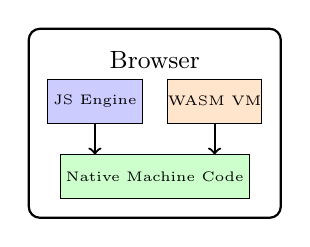
\begin{tikzpicture}[scale=0.8]
    % Browser box
    \draw[thick, rounded corners] (0,0) rectangle (4,3);
    \node at (2,2.5) {\small Browser};
    
    % JS Engine
    \draw[fill=blue!20] (0.3,1.5) rectangle (1.8,2.2);
    \node at (1.05,1.85) {\tiny JS Engine};
    
    % WASM VM
    \draw[fill=orange!20] (2.2,1.5) rectangle (3.7,2.2);
    \node at (2.95,1.85) {\tiny WASM VM};
    
    % Native Code
    \draw[fill=green!20] (0.5,0.3) rectangle (3.5,1);
    \node at (2,0.65) {\tiny Native Machine Code};
    
    % Arrows
    \draw[->, thick] (1.05,1.5) -- (1.05,1);
    \draw[->, thick] (2.95,1.5) -- (2.95,1);
\end{tikzpicture}
\end{columns}
\end{frame}

\begin{frame}{Key Features of WebAssembly}
\begin{itemize}
    \item \textbf{Fast}: Near-native execution speed
    \item \textbf{Safe}: Memory-safe, sandboxed execution environment
    \item \textbf{Open}: Open web standard, platform-independent
    \item \textbf{Portable}: Single .wasm file runs anywhere
    \item \textbf{Compact}: Binary format, smaller than JavaScript
    \item \textbf{Polyglot}: Compile from C/C++, Rust, Go, etc.
\end{itemize}
\end{frame}

\begin{frame}[fragile]{WebAssembly Text Format (WAT)}
\begin{lstlisting}[language=Lisp]
(module
  (func $add (param $a i32) (param $b i32) (result i32)
    local.get $a
    local.get $b
    i32.add)
  (export "add" (func $add))
)
\end{lstlisting}

Compiles to binary format:
\begin{lstlisting}
00 61 73 6d 01 00 00 00 01 07 01 60 02 7f 7f 01
7f 03 02 01 00 07 07 01 03 61 64 64 00 00 0a 09
01 07 00 20 00 20 01 6a 0b
\end{lstlisting}
\end{frame}

% Section 2: WASI
\section{WASI - WebAssembly System Interface}

\begin{frame}{What is WASI?}
\begin{block}{Definition}
WebAssembly System Interface (WASI) is a modular system interface for WebAssembly that enables WASM modules to interact with the operating system.
\end{block}

\begin{itemize}
    \item Standardized API for system calls
    \item Platform-agnostic interface
    \item Capability-based security model
    \item Write once, run anywhere (beyond browsers)
\end{itemize}
\end{frame}

\begin{frame}{WASI Architecture}
\begin{center}
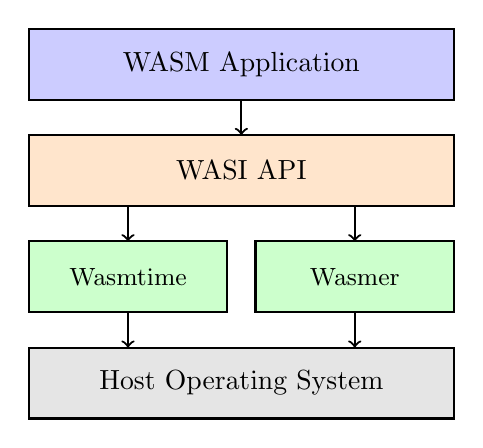
\begin{tikzpicture}[scale=0.9]
    % Application layer
    \draw[thick, fill=blue!20] (0,4) rectangle (6,5);
    \node at (3,4.5) {WASM Application};
    
    % WASI layer
    \draw[thick, fill=orange!20] (0,2.5) rectangle (6,3.5);
    \node at (3,3) {WASI API};
    
    % Runtime layer
    \draw[thick, fill=green!20] (0,1) rectangle (2.8,2);
    \draw[thick, fill=green!20] (3.2,1) rectangle (6,2);
    \node at (1.4,1.5) {\small Wasmtime};
    \node at (4.6,1.5) {\small Wasmer};
    
    % OS layer
    \draw[thick, fill=gray!20] (0,-0.5) rectangle (6,0.5);
    \node at (3,0) {Host Operating System};
    
    % Arrows
    \draw[->, thick] (3,4) -- (3,3.5);
    \draw[->, thick] (1.4,2.5) -- (1.4,2);
    \draw[->, thick] (4.6,2.5) -- (4.6,2);
    \draw[->, thick] (1.4,1) -- (1.4,0.5);
    \draw[->, thick] (4.6,1) -- (4.6,0.5);
\end{tikzpicture}
\end{center}
\end{frame}

\begin{frame}[fragile]{WASI Capabilities}
\begin{columns}
\column{0.5\textwidth}
Core WASI APIs:
\begin{itemize}
    \item File system access
    \item Environment variables
    \item Clock/Time functions
    \item Random number generation
    \item Process exit codes
    \item Standard I/O streams
\end{itemize}

\column{0.5\textwidth}
\begin{lstlisting}[language=C]
#include <stdio.h>
#include <stdlib.h>

int main() {
    // WASI file system
    FILE *f = fopen("data.txt", "r");
    
    // WASI environment
    char *path = getenv("PATH");
    
    // WASI random
    int r = rand();
    
    return 0;
}
\end{lstlisting}
\end{columns}
\end{frame}

% Section 3: WASIX
\section{WASIX - Extended WASI}

\begin{frame}{What is WASIX?}
\begin{block}{WASIX Definition}
WASIX is a superset of WASI that extends the standard with additional POSIX-compatible system calls, enabling more complex applications to run in WebAssembly.
\end{block}

Key additions:
\begin{itemize}
    \item Full POSIX threading support
    \item Network sockets (TCP/UDP)
    \item Process forking and execution
    \item Shared memory
    \item Signal handling
    \item Extended file system operations
\end{itemize}
\end{frame}

\begin{frame}{WASI vs WASIX Comparison}
\begin{center}
\begin{tabular}{|l|c|c|}
\hline
\textbf{Feature} & \textbf{WASI} & \textbf{WASIX} \\
\hline
File I/O & \checkmark & \checkmark \\
Environment Variables & \checkmark & \checkmark \\
Random Numbers & \checkmark & \checkmark \\
Clocks/Time & \checkmark & \checkmark \\
\hline
Threading & Limited & \checkmark Full \\
Networking & $\times$ & \checkmark \\
Fork/Exec & $\times$ & \checkmark \\
Signals & $\times$ & \checkmark \\
Shared Memory & $\times$ & \checkmark \\
Futex & $\times$ & \checkmark \\
\hline
\end{tabular}
\end{center}
\end{frame}

\begin{frame}[fragile]{WASIX Example: Threading}
\begin{lstlisting}[language=C]
#include <pthread.h>
#include <stdio.h>

void* worker(void* arg) {
    int id = *(int*)arg;
    printf("Thread %d running\n", id);
    return NULL;
}

int main() {
    pthread_t threads[4];
    int thread_ids[4];
    
    for (int i = 0; i < 4; i++) {
        thread_ids[i] = i;
        pthread_create(&threads[i], NULL, 
                      worker, &thread_ids[i]);
    }
    
    for (int i = 0; i < 4; i++) {
        pthread_join(threads[i], NULL);
    }
    
    return 0;
}
\end{lstlisting}
\end{frame}

% Section 4: Architecture and Design
\section{Architecture and Design Principles}

\begin{frame}{WebAssembly Architecture}
\begin{center}
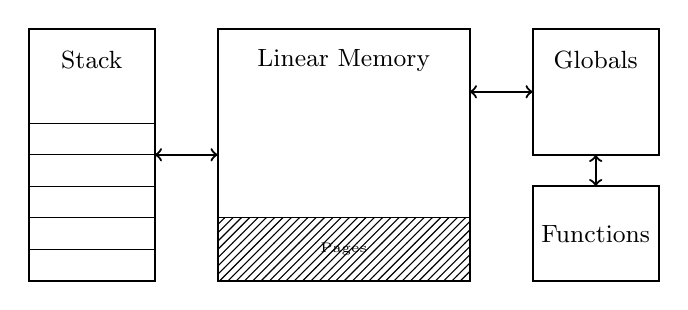
\begin{tikzpicture}[scale=0.8]
    % Stack Machine
    \draw[thick] (0,0) rectangle (2,4);
    \node at (1,3.5) {\small Stack};
    \foreach \y in {0.5,1,1.5,2,2.5} {
        \draw (0,\y) -- (2,\y);
    }
    
    % Linear Memory
    \draw[thick] (3,0) rectangle (7,4);
    \node at (5,3.5) {\small Linear Memory};
    \draw[pattern=north east lines] (3,0) rectangle (7,1);
    \node at (5,0.5) {\tiny Pages};
    
    % Globals
    \draw[thick] (8,2) rectangle (10,4);
    \node at (9,3.5) {\small Globals};
    
    % Functions
    \draw[thick] (8,0) rectangle (10,1.5);
    \node at (9,0.75) {\small Functions};
    
    % Arrows
    \draw[<->, thick] (2,2) -- (3,2);
    \draw[<->, thick] (7,3) -- (8,3);
    \draw[<->, thick] (9,1.5) -- (9,2);
\end{tikzpicture}
\end{center}

Key Components:
\begin{itemize}
    \item Stack-based virtual machine
    \item Linear memory model (pages of 64KB)
    \item Global variables
    \item Function imports/exports
\end{itemize}
\end{frame}

\begin{frame}{Security Model}
\begin{columns}
\column{0.5\textwidth}
\textbf{Sandboxing}
\begin{itemize}
    \item Memory isolation
    \item No direct system calls
    \item Capability-based access
    \item Explicit imports/exports
\end{itemize}

\textbf{WASI Capabilities}
\begin{itemize}
    \item File descriptors
    \item Directory handles
    \item Network sockets (WASIX)
    \item Granular permissions
\end{itemize}

\column{0.5\textwidth}
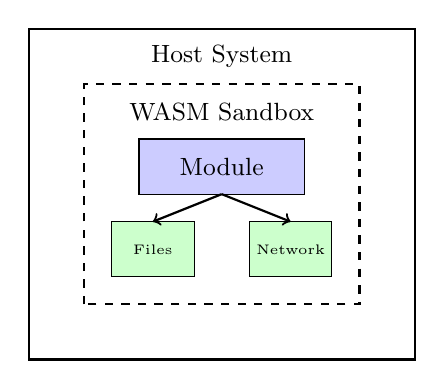
\begin{tikzpicture}[scale=0.7]
    % Sandbox
    \draw[thick, dashed] (0,0) rectangle (5,4);
    \node at (2.5,3.5) {\small WASM Sandbox};
    
    % Module
    \draw[fill=blue!20] (1,2) rectangle (4,3);
    \node at (2.5,2.5) {\small Module};
    
    % Capabilities
    \draw[fill=green!20] (0.5,0.5) rectangle (2,1.5);
    \draw[fill=green!20] (3,0.5) rectangle (4.5,1.5);
    \node at (1.25,1) {\tiny Files};
    \node at (3.75,1) {\tiny Network};
    
    % Arrows
    \draw[->, thick] (2.5,2) -- (1.25,1.5);
    \draw[->, thick] (2.5,2) -- (3.75,1.5);
    
    % Host
    \draw[thick] (-1,-1) rectangle (6,5);
    \node at (2.5,4.5) {\small Host System};
\end{tikzpicture}
\end{columns}
\end{frame}

% Section 5: Use Cases
\section{Use Cases and Applications}

\begin{frame}{WebAssembly Use Cases}
\begin{columns}
\column{0.5\textwidth}
\textbf{Browser Applications}
\begin{itemize}
    \item Games and graphics
    \item Video/audio processing
    \item CAD applications
    \item Scientific computing
    \item Cryptocurrency wallets
\end{itemize}

\column{0.5\textwidth}
\textbf{Server-Side Applications}
\begin{itemize}
    \item Edge computing
    \item Serverless functions
    \item Plugin systems
    \item Embedded systems
    \item Blockchain smart contracts
\end{itemize}
\end{columns}

\vspace{0.5cm}
\begin{center}
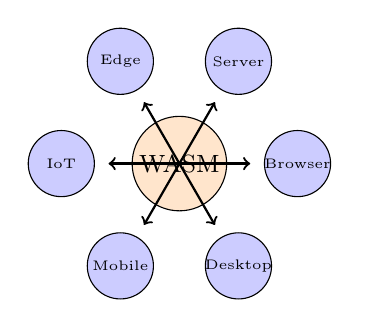
\begin{tikzpicture}[scale=0.6]
    % Center
    \draw[fill=orange!20] (0,0) circle (1cm);
    \node at (0,0) {\small WASM};
    
    % Surrounding nodes
    \foreach \angle/\label in {0/Browser, 60/Server, 120/Edge, 180/IoT, 240/Mobile, 300/Desktop} {
        \draw[fill=blue!20] (\angle:2.5) circle (0.7cm);
        \node at (\angle:2.5) {\tiny \label};
        \draw[->, thick] (0,0) -- (\angle:1.5);
    }
\end{tikzpicture}
\end{center}
\end{frame}

\begin{frame}{Real-World Examples}
\begin{itemize}
    \item \textbf{Figma}: Design tool running in browser via WASM
    \item \textbf{AutoCAD}: Web version powered by WebAssembly
    \item \textbf{Cloudflare Workers}: Serverless computing with WASM
    \item \textbf{Fastly Compute@Edge}: Edge computing platform
    \item \textbf{Docker Desktop}: Uses WASM for extensions
    \item \textbf{Krustlet}: Kubernetes kubelet for WASM workloads
    \item \textbf{Wasmer}: Universal WASM runtime with WASIX
\end{itemize}
\end{frame}

% Section 6: Performance
\section{Performance Characteristics}

\begin{frame}{Performance Comparison}
\begin{center}
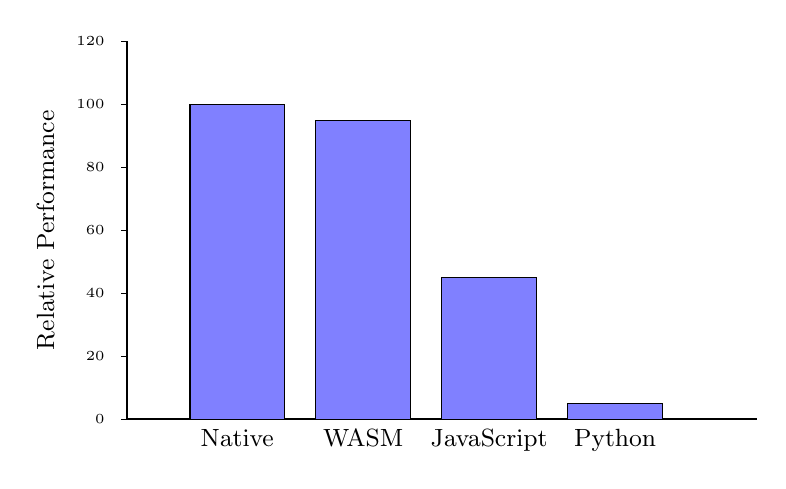
\begin{tikzpicture}[scale=0.8]
    % Manual bar chart
    \draw[thick] (0,0) -- (10,0); % x-axis
    \draw[thick] (0,0) -- (0,6); % y-axis
    
    % Y-axis labels
    \foreach \y/\label in {0/0, 1/20, 2/40, 3/60, 4/80, 5/100, 6/120} {
        \draw (0,\y) -- (-0.1,\y);
        \node[left] at (-0.2,\y) {\tiny \label};
    }
    
    % Bars
    \draw[fill=blue!50] (1,0) rectangle (2.5,5);    % Native (100)
    \draw[fill=blue!50] (3,0) rectangle (4.5,4.75); % WASM (95)
    \draw[fill=blue!50] (5,0) rectangle (6.5,2.25); % JavaScript (45)
    \draw[fill=blue!50] (7,0) rectangle (8.5,0.25); % Python (5)
    
    % X-axis labels
    \node[below] at (1.75,0) {\small Native};
    \node[below] at (3.75,0) {\small WASM};
    \node[below] at (5.75,0) {\small JavaScript};
    \node[below] at (7.75,0) {\small Python};
    
    % Y-axis label
    \node[rotate=90, above] at (-1,3) {\small Relative Performance};
\end{tikzpicture}
\end{center}

\small
*Benchmark: Computational intensive tasks (approximate values)
\end{frame}

\begin{frame}{Performance Factors}
\begin{columns}
\column{0.5\textwidth}
\textbf{Advantages}
\begin{itemize}
    \item Ahead-of-time compilation
    \item Predictable performance
    \item No garbage collection pauses
    \item Efficient memory usage
    \item SIMD instructions support
\end{itemize}

\column{0.5\textwidth}
\textbf{Considerations}
\begin{itemize}
    \item Startup overhead
    \item Memory copy costs
    \item JavaScript interop overhead
    \item Limited threading (WASI)
    \item Module size
\end{itemize}
\end{columns}
\end{frame}

% Section 7: Future
\section{Future Developments}

\begin{frame}{WebAssembly Roadmap}
\textbf{Current Proposals}
\begin{itemize}
    \item \textbf{Component Model}: Composable WASM modules
    \item \textbf{Interface Types}: Better language interop
    \item \textbf{GC Support}: Garbage collected languages
    \item \textbf{Exception Handling}: Native exception support
    \item \textbf{Tail Calls}: Functional programming optimization
\end{itemize}

\textbf{WASI Evolution}
\begin{itemize}
    \item WASI Preview 2: Component model integration
    \item Standardized networking APIs
    \item GPU access proposals
    \item Improved async/await support
\end{itemize}
\end{frame}

\begin{frame}{Future Vision}
\begin{center}
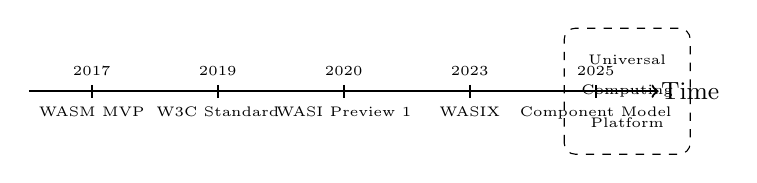
\begin{tikzpicture}[scale=0.8]
    % Timeline
    \draw[thick, ->] (0,0) -- (10,0);
    \node at (10.5,0) {\small Time};
    
    % Milestones
    \foreach \x/\year/\label in {1/2017/{WASM MVP}, 3/2019/{W3C Standard}, 5/2020/{WASI Preview 1}, 7/2023/{WASIX}, 9/2025/{Component Model}} {
        \draw[thick] (\x,0.1) -- (\x,-0.1);
        \node[above] at (\x,0.1) {\tiny \year};
        \node[below, align=center] at (\x,-0.1) {\tiny \label};
    }
    
    % Future box
    \draw[dashed, rounded corners] (8.5,-1) rectangle (10.5,1);
    \node at (9.5,0.5) {\tiny Universal};
    \node at (9.5,0) {\tiny Computing};
    \node at (9.5,-0.5) {\tiny Platform};
\end{tikzpicture}
\end{center}

\textbf{Vision}: Write once, run anywhere
\begin{itemize}
    \item Universal application runtime
    \item Language-agnostic platform
    \item Seamless cloud-to-edge deployment
    \item Native performance everywhere
\end{itemize}
\end{frame}

\begin{frame}{Conclusion}
\begin{itemize}
    \item \textbf{WASM}: Efficient, portable bytecode format
    \item \textbf{WASI}: System interface for non-browser environments
    \item \textbf{WASIX}: Extended POSIX compatibility
    \item Growing ecosystem with broad industry support
    \item Promising future for universal computing
\end{itemize}

\vspace{0.5cm}
\begin{center}
\Large Thank You!

\vspace{0.5cm}
\normalsize
Questions?
\end{center}
\end{frame}

\begin{frame}{Resources}
\begin{itemize}
    \item \textbf{WebAssembly.org}: \url{https://webassembly.org/}
    \item \textbf{WASI.dev}: \url{https://wasi.dev/}
    \item \textbf{Wasmer.io}: \url{https://wasmer.io/}
    \item \textbf{MDN WebAssembly}: \url{https://developer.mozilla.org/en-US/docs/WebAssembly}
    \item \textbf{WASM Weekly}: Newsletter for WebAssembly updates
    \item \textbf{Awesome WebAssembly}: Curated list of resources
\end{itemize}
\end{frame}

\end{document}